Em \python, a melhor forma de ser representar os dados para análise gráfica costuma ser com as ferramentas do \pandas. Nessa biblioteca os dados são tratados na forma de um \dataframe, um tipo de representação de um tabela com a mesma abstração de linhas e colunas. Essa tabela pode ser construída manualmente ou gerada de um arquivo de texto ou binário seguindo algumas especificações. As colunas do \dataframe são acessadas por nome, similar ao acesso por chave em um dicionáro.

No caso dos dados de um gerenciador de tabelas, como o \texttt{Excel}, o \texttt{Google Planilhas} ou o \texttt{LibreOffice Calc}, é preciso organizar os valores em colunas, como na figura \ref{fig:basico:dados}, em uma folha de planilha própria com apenas estes dados. É recomendável, também, colocar estes dados no começo da folha, começando na primeira linha e na primeira coluna, e deixar a primeira linha dos dados com o nome da coluna que será usado para acesso no \dataframe.

\begin{figure}[H]
    \centering
    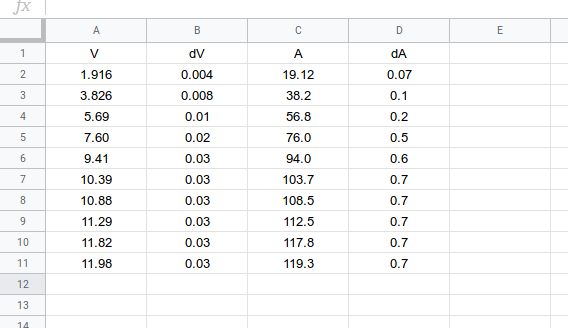
\includegraphics[width=0.7\textwidth]{basico/dados.png}

    \caption{Organização dos dados para importar em \python}
    \label{fig:basico:dados}
\end{figure}


\subsubsection{Arquivos CSV}

    Arquivos \texttt{CSV} (\textit{Comma Separated Values}) são os mais típicos para armazenamento de dados para análises. Eles são basicamente arquivos de textos, então podem ser visualizados e editados em qualquer editor de texto, mas os valores são separados por algum carácter específico, normalmente a vírgula (\texttt{,}), e as primeiras linhas podem ser utilizadas como \textit{header} dos dados.

    \begin{figure}[H]
        \centering
        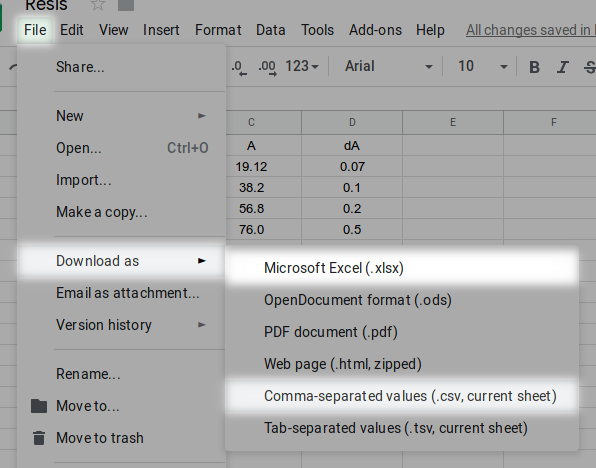
\includegraphics[width=0.6\textwidth]{basico/download.png}

        \caption{Recuperando os valores de uma folha de planilha no Google Planilhas}
        \label{fig:basico:download}
    \end{figure}

    Apesar de o exemplo da figura \ref{fig:basico:download} ser apenas no \texttt{Google Planilhas}, qualquer outro gerenciador de tabelas atual terá uma opção similar como parte do programa também. Uma vez que o \texttt{CSV} esteja pronto, ele pode ser transformado em um \dataframe com a função \href{http://pandas.pydata.org/pandas-docs/stable/reference/api/pandas.read_csv.html#pandas.read_csv}{\pyline{read_csv}} do \pandas.

    O argumento \pyline{decimal} da função representa qual o carácter a ser entendido como separador decimal. No exemplo do código \ref{code:basico:csv}, é usado a vírgula como separador, mas se por acaso estiver usando o ponto final para isso, lembre-se de mudar para \pyline{'.'}. Se o separador estiver diferente, o \pandas vai entender o valor como texto, o que não servirá para a montagem do gráfico depois.

    \begin{listing}[H]
        \caption{Leitura de um \dataframe a partir de um \texttt{CSV}}
        \label{code:basico:csv}

        \pyinclude[firstline=3,lastline=5]{recursos/basico/read.py}
    \end{listing}


\subsubsection{Arquivos do Excel}

    Também é possível ler diretamente arquivos do \texttt{Excel} ou arquivos do mesmo tipo (\texttt{.xlsx}) extraído de outro programa, como na figura \ref{fig:basico:download}. Para isso, além de expecificar o nome do arquivo, é necessário dizer qual a folha da planilha a ser usada com o argumento \pyline{sheet_name}, como no código \ref{code:basico:xlsx}, tudo com a função \href{http://pandas.pydata.org/pandas-docs/stable/reference/api/pandas.read_excel.html#pandas.read_excel}{\pyline{read_excel}}. Para este tipo de arquivo, não precisa preocupar com o separador de decimal, pois a representação interna do dado já é númerica, em vez de textual, como era no \texttt{CSV}.

    \begin{listing}[H]
        \caption{Leitura de um \dataframe a partir de um arquivo de \texttt{Excel}}
        \label{code:basico:xlsx}

        \pyinclude[firstline=7,lastline=9]{recursos/basico/read.py}
    \end{listing}
